\documentclass[12pt, xcolor=table]{beamer}

\usepackage{geometry}

\usepackage{lmodern}
\usepackage[utf8]{inputenc}
\usepackage[T1]{fontenc}		
\usepackage[english]{babel}

\usepackage{siunitx}

\usepackage{xcolor, colortbl}
\definecolor{darkgreen}{RGB}{0, 155, 85}
\definecolor{elancourt}{rgb}{1,.79,.5}
\definecolor{paris}{rgb}{.84,.1,.11}
\definecolor{nantes}{rgb}{.17,.51,.73}

\renewcommand<>\cellcolor[1]{\only#2{\beameroriginal\cellcolor{#1}}}

\definecolor{LOSS35}{RGB}{255,0,0}
\definecolor{LOSS1535}{RGB}{255,122,12}
\definecolor{LOSS0515}{RGB}{255,181,12}
\definecolor{STBL}{RGB}{58,255,12}
\definecolor{GAIN0515}{RGB}{58,178,12}
\definecolor{GAIN1535}{RGB}{56,136,17}
\definecolor{GAIN35}{RGB}{50,119,16}


\usepackage{graphicx}
\usepackage{floatrow}
\usepackage[
    scriptsize,
    labelformat=empty
]{caption}

\usepackage{tcolorbox}

\usepackage{enumitem}

\usepackage{standalone}

\usepackage{multirow}

\usepackage{array}
\newcolumntype{x}[1]{>{\centering\let\newline\\\arraybackslash\hspace{0pt}}m{#1}}
\usepackage{booktabs}
\usepackage{makecell}

\usepackage{tikz}
\usetikzlibrary{calc, 3d, shadows, decorations, shapes, fadings, trees, backgrounds, fit, patterns}
\usepackage{pgfplots}
\usepackage{pgfplotstable}
\usepgfplotslibrary{groupplots}
\usepackage{forest}
\usepackage[final]{animate}

\usepackage{amsmath}
\usepackage{amsthm}
\usepackage{amsfonts}
\usepackage{amssymb}
\usepackage{mathrsfs}
\usepackage{bm}
\usepackage{bbold}
\usepackage{stmaryrd}
\usepackage{mleftright}
    
\usepackage[
    backend=biber,
    style=authoryear,
    dashed=false,
    sorting=nty,
    maxbibnames=5,
    minbibnames=5,
    maxcitenames=1,
    uniquelist=false,
    uniquename=false,
    hyperref=true,
    backref=true,
    backrefstyle=all+,
    isbn=false,
    url=false,
    doi=false
]{biblatex}
\usepackage{xpatch}

\addbibresource{references.bib}

\usepackage[acronym, toc, automake=true]{glossaries}

\usepackage{hyperref}
\hypersetup{
    pdftitle={Semantic aware quality evaluation of 3D building models},
    pdfauthor={Oussama Ennafii},
    pdfkeywords={3D urban modeling} {buildings} {quality assessment} {taxonomy} {classification} {error detection} {geometry} {aerial imagery} {Very High Spatial Resolution} {Digital Surface Model},
    pdfstartview={FitH},
    unicode=true
}

\setbeamerfont{footnote}{size=\tiny}

\tikzset{
    invisible/.style={opacity=0},
    visible on/.style={alt=#1{}{invisible}},
    alt/.code args={<#1>#2#3}{
        \alt<#1>{\pgfkeysalso{#2}}{\pgfkeysalso{#3}}
    },
}

\NewDocumentCommand{\evalat}{sO{\big}mm}{%
    \IfBooleanTF{#1}
    {\mleft. #3 \mright|_{#4}}
    {#3#2|_{#4}}%
}
\makeatletter
\newcommand{\ostar}{\mathbin{\mathpalette\make@circled\star}}
\newcommand{\make@circled}[2]{%
    \ooalign{$\m@th#1\smallbigcirc{#1}$\cr\hidewidth$\m@th#1#2$\hidewidth\cr}%
}
\newcommand{\smallbigcirc}[1]{%
    \vcenter{\hbox{\scalebox{0.77778}{$\m@th#1\bigcirc$}}}%
}

\patchcmd{\beamer@sectionintoc}{\vskip1.5em}{\vskip0.5em}{}{}

\makeatother


\usepackage[useregional]{datetime2}

\usepackage{style/glossaries}

\usetheme{ign}

\title{Quality evaluation of 3D building models}
\subtitle{A scalable approach}
\date{\tiny \DTMdisplaydate{2020}{10}{08}{5}}
\author{
    Oussama Ennafii
}

\institute{
    Univ. Paris Est, LaSTIG STRUDEL
    \and
    Gambi-M
}

\begin{document}
    \begin{frame}[plain]
        \titlepage
    \end{frame}

    \section{Introduction}
        \subsection{Context}
            \begin{frame}{Reconstruction \texttt{vs.} Modeling}
                \centering
                \begin{columns}[T]
                    \footnotesize
                    \begin{column}{.5\textwidth}
                        \begin{center}
                            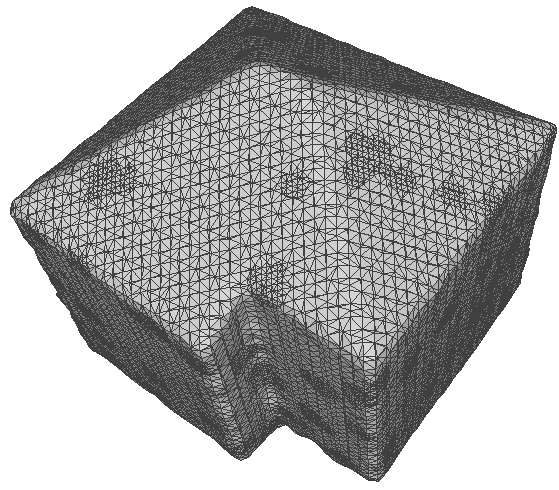
\includegraphics[width=.48\linewidth]{images/mesh_model/mesh}
                        \end{center}

                        \begin{itemize}[label=\(\blacktriangleright\), font=\color{IGNGreen}]
                            \item<1-> Surface reconstruction.
                            \item[\color{IGNGreen} +]<2-> \textcolor{IGNGreen}{High geometric fidelity.}
                            \item[\color{IGNRed} ---]<2-> \textcolor{IGNRed}{Low compactness.}
                        \end{itemize}
                    \end{column}
                    \begin{column}{.5\textwidth}
                        \uncover<3->{
                            \begin{center}
                                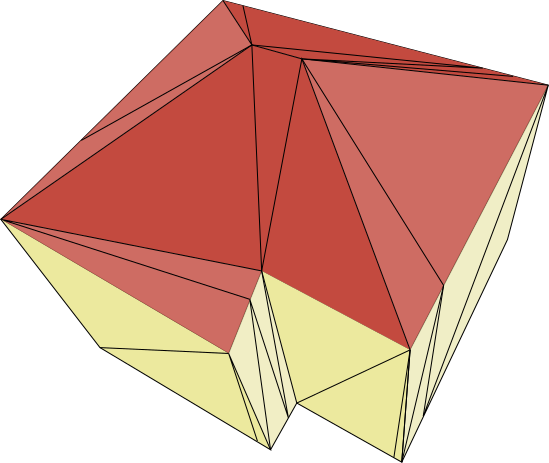
\includegraphics[width=.48\linewidth]{images/mesh_model/model}
                            \end{center}
                        }

                        \begin{itemize}[label=\(\blacktriangleright\), font=\color{IGNGreen}]
                            \item<3-> Modeling.
                            \item[\color{IGNRed} ---]<4->\textcolor{IGNRed}{Low geometric fidelity.}
                            \item[\color{IGNGreen} +]<4-> \textcolor{IGNGreen}{High compactness.}
                        \end{itemize}
                    \end{column}
                \end{columns}
                \vfill
                \begin{itemize}[label=\(\blacktriangleright\), font=\color{IGNGreen}]
                    \item<5-> Literature: trade off fidelity/compactness.
                \end{itemize}
            \end{frame}

            \begin{frame}{Modeling}{Multiple sources of errors}
                \begin{itemize}[label=\(\blacktriangleright\), font=\color{IGNGreen}, itemsep=2em]
                    \item<1-> Input imprecision: footprints, depth maps \dots
                    \item<2-> High (inter-) variance between building types;
                    \item<3-> High (intra-) variance between features inside a building;
                \end{itemize}
            \end{frame}
        
        \subsection{Quality evaluation}            
            \begin{frame}{Our wish list}
                \begin{itemize}[label=\(\blacktriangleright\), font=\color{IGNGreen}, itemsep=1em]
                    \item<1-> \textbf{Scalability} up to city level (> \num{10000} buildings);
                    \item<2-> \underline{Genericity} towards:
                    \begin{enumerate}[label=(\roman*)]
                        \item<3-> modeling approach of origin;
                        \item<4-> urban scene.
                    \end{enumerate}
                    \item<5-> Readily available reference data;
                    \item<6-> \textbf{Automation}: no human intervention.
                \end{itemize}
            \end{frame}

            \begin{frame}{Our approach}
                \begin{enumerate}[label=\arabic* --, itemsep=2em, font=\color{IGNGreen}]
                    \item<1-> Semantic error taxonomy~\parencite{ennafii2019learning};
                    \item<2-> Learning based evaluation approach;
                    \item<3-> An efficient representation of \acrshort{acr::3d} building models.
                \end{enumerate}
            \end{frame}

    \AtBeginSection[]{
        \begin{frame}<beamer>
            \frametitle{Outline}
            \tableofcontents[currentsubsection, subsectionstyle=show/show/hide]
        \end{frame}
    }

    \section{Learning based evaluation}
        \subsection{Error taxonomy}
            \begin{frame}{Atomic errors}{Under segmentation}
                \begin{itemize}[label=\(\blacktriangleright\), font=\color{IGNGreen}]
                    \item<1-> \Acrfull{acr::2d} errors:
                    \begin{itemize}[label=\(\blacktriangleright\), font=\color{IGNGreen}]
                        \item<2-> Segmentation issue:
                        \begin{itemize}
                            \item<3-> Under segmentation: \only<3>{building level}\only<4>{facet level};
                        \end{itemize}
                    \end{itemize}
                \end{itemize}
                \begin{overlayarea}{\textwidth}{.5\textheight}
                    \only<3->{
                        \begin{columns}[T]
                            \begin{column}{.5\textwidth}
                                \centering
                                \begin{figure}[H]
                                    \centering
                                    \alt<3>{
                                        \includestandalone[mode=buildnew, height=.4\textheight]{figures/errors/building/bos}
                                    }{
                                        \includestandalone[mode=buildnew, height=.4\textheight]{figures/errors/facet/correct_fos_fus_fib_fig}
                                    }
                                    \caption{Ground truth.}
                                \end{figure}
                            \end{column}
                            \begin{column}{.5\textwidth}
                                \begin{figure}[H]
                                    \centering
                                    \alt<3>{
                                        \includestandalone[mode=buildnew, height=.4\textheight]{figures/errors/building/bus}
                                    }{
                                        \includestandalone[mode=buildnew, height=.4\textheight]{figures/errors/facet/fus}
                                    }
                                    \caption{Model.}
                                \end{figure}
                            \end{column}
                        \end{columns}
                    }
                \end{overlayarea}
            \end{frame}

            \begin{frame}{Atomic errors}{Over segmentation}
                \begin{itemize}[label=\(\blacktriangleright\), font=\color{IGNGreen}]
                    \item \Acrfull{acr::2d} errors:
                    \begin{itemize}[label=\(\blacktriangleright\), font=\color{IGNGreen}]
                        \item Segmentation issue:
                        \begin{itemize}
                            \item<1-> Over segmentation: \only<1>{building level}\only<2>{facet level}.
                        \end{itemize}
                    \end{itemize}
                \end{itemize}
                \begin{overlayarea}{\textwidth}{.5\textheight}
                    \only<1->{
                        \begin{columns}[T]
                            \begin{column}{.5\textwidth}
                                \centering
                                \begin{figure}[H]
                                    \centering
                                    \alt<1>{
                                        \includestandalone[mode=buildnew, height=.4\textheight]{figures/errors/building/bus}
                                    }{
                                        \includestandalone[mode=buildnew, height=.4\textheight]{figures/errors/facet/correct_fos_fus_fib_fig}
                                    }
                                    \caption{Ground truth.}
                                \end{figure}
                            \end{column}
                            \begin{column}{.5\textwidth}
                                \begin{figure}[H]
                                    \centering
                                    \alt<1>{
                                        \includestandalone[mode=buildnew, height=.4\textheight]{figures/errors/building/bos}
                                    }{
                                        \includestandalone[mode=buildnew, height=.4\textheight]{figures/errors/facet/fos}
                                    }
                                    \caption{Model.}
                                \end{figure}
                            \end{column}
                        \end{columns}
                    }
                \end{overlayarea}
            \end{frame}

            \begin{frame}{Atomic errors}{Inaccurate topology}
                \begin{itemize}[label=\(\blacktriangleright\), font=\color{IGNGreen}]
                    \item<1-> \Acrfull{acr::2d} errors:
                    \begin{itemize}[label=\(\blacktriangleright\), font=\color{IGNGreen}]
                        \item<2-> Border issue:
                        \begin{itemize}
                            \item<3-4> Inaccurate topology: \only<3>{building level}\only<4>{facet level};
                        \end{itemize}
                    \end{itemize}
                \end{itemize}
                \begin{overlayarea}{\textwidth}{.5\textheight}
                    \only<3->{
                        \begin{columns}[T]
                            \begin{column}{.5\textwidth}
                                \centering
                                \begin{figure}[H]
                                    \centering
                                    \alt<3>{
                                        \includestandalone[mode=buildnew, height=.4\textheight]{figures/errors/building/correct_bit}
                                    }{
                                        \includestandalone[mode=buildnew, height=.4\textheight]{figures/errors/facet/correct_fit}
                                    }
                                    \caption{Ground truth.}
                                \end{figure}
                            \end{column}
                            \begin{column}{.5\textwidth}
                                \begin{figure}[H]
                                    \centering
                                    \alt<3>{
                                        \includestandalone[mode=buildnew, height=.4\textheight]{figures/errors/building/bit}
                                    }{
                                        \includestandalone[mode=buildnew, height=.4\textheight]{figures/errors/facet/fit}
                                    }
                                    \caption{Model.}
                                \end{figure}
                            \end{column}
                        \end{columns}
                    }
                \end{overlayarea}
            \end{frame}

            \begin{frame}{Atomic errors}{Imprecise border}
                \begin{itemize}[label=\(\blacktriangleright\), font=\color{IGNGreen}]
                    \item \Acrfull{acr::2d} errors:
                    \begin{itemize}[label=\(\blacktriangleright\), font=\color{IGNGreen}]
                        \item Border issue:
                        \begin{itemize}
                            \item<1-> Imprecise border: \only<1>{building level}\only<2>{facet level}.
                        \end{itemize}
                    \end{itemize}
                \end{itemize}
                \begin{overlayarea}{\textwidth}{.5\textheight}
                    \only<1->{
                        \begin{columns}[T]
                            \begin{column}{.5\textwidth}
                                \centering
                                \begin{figure}[H]
                                    \centering
                                    \alt<1>{
                                        \includestandalone[mode=buildnew, height=.38\textheight]{figures/errors/building/correct_bib}
                                    }{
                                        \includestandalone[mode=buildnew, height=.4\textheight]{figures/errors/facet/correct_fos_fus_fib_fig}
                                    }
                                    \caption{Ground truth.}
                                \end{figure}
                            \end{column}
                            \begin{column}{.5\textwidth}
                                \begin{figure}[H]
                                    \centering
                                    \alt<1>{
                                        \includestandalone[mode=buildnew, height=.4\textheight]{figures/errors/building/bib}
                                    }{
                                        \includestandalone[mode=buildnew, height=.4\textheight]{figures/errors/facet/fib}
                                    }
                                    \caption{Model.}
                                \end{figure}
                            \end{column}
                        \end{columns}
                    }
                \end{overlayarea}
            \end{frame}

            \begin{frame}{Atomic errors}{\texorpdfstring{\acrshort*{acr::3d}}{3D} errors}
                \begin{itemize}[label=\(\blacktriangleright\), font=\color{IGNGreen}]
                    \item<1-> \Acrfull{acr::3d} errors:
                    \begin{itemize}[label=\(\blacktriangleright\), font=\color{IGNGreen}]
                        \item<2-3> Imprecise geometry: \only<2>{building level}\only<3>{facet level}.
                        \begin{itemize}
                            \item 
                        \end{itemize}
                    \end{itemize}
                \end{itemize}
                \begin{overlayarea}{\textwidth}{.5\textheight}
                    \only<2->{
                        \begin{columns}[T]
                            \begin{column}{.5\textwidth}
                                \centering
                                \begin{figure}[H]
                                    \centering
                                    \alt<2>{
                                        \includestandalone[mode=buildnew, height=.4\textheight]{figures/errors/building/correct_big}
                                    }{
                                        \includestandalone[mode=buildnew, height=.4\textheight]{figures/errors/facet/correct_fos_fus_fib_fig}
                                    }
                                    \caption{Ground truth.}
                                \end{figure}
                            \end{column}
                            \begin{column}{.5\textwidth}
                                \begin{figure}[H]
                                    \centering
                                    \alt<2>{
                                        \includestandalone[mode=buildnew, height=.4\textheight]{figures/errors/building/big}
                                    }{
                                        \includestandalone[mode=buildnew, height=.4\textheight]{figures/errors/facet/fig}
                                    }
                                    \caption{Model.}
                                \end{figure}
                            \end{column}
                        \end{columns}
                    }
                \end{overlayarea}
            \end{frame}

        \subsection{Evaluation workflow}
            \begin{frame}{Evaluation as classification}
                \begin{itemize}[label=$\blacktriangleright$, font=\color{IGNGreen}]
                    \item<1-> Error detection \(\longleftrightarrow\) \textbf{supervised classification}:
                    \begin{itemize}[label=\(\rightarrow\)]
                        \item<2-> Adapted to \textbf{large scales};
                        \item<3-> \textbf{Automated} by design.
                    \end{itemize}
                    \item<4-> No hierarchy between \texttt{atomic errors}:
                    \begin{itemize}[label=$\implies$]
                        \item<5-> Multilabel classification.
                    \end{itemize}
                    \item<6-> Evaluation at \underline{building level};
                \end{itemize}
            \end{frame}

            \begin{frame}{Generic workflow}
                \centering
                \includestandalone[mode=buildnew, height=.75\textheight]{figures/graphical_pipeline}
            \end{frame}

    \section{An efficient representation}
        \subsection{Geometric features}
            \begin{frame}{Models as graphs}
                \centering
                \includestandalone[mode=buildnew, width=.7\textwidth]{figures/features/geometric/graph_animated}
                \begin{itemize}[label=$\blacktriangleright$, font=\color{IGNGreen}]
                    \item Graph = \only<2->{\textcolor{darkgreen}{nodes(facets)}} \only<3->{ + \textcolor{blue}{edges(adjacency)}.}
                \end{itemize}
            \end{frame}

        \subsection{Image features}            
            \begin{frame}{Height based features}
                \centering
                \includestandalone[mode=buildnew, width=\textwidth]{figures/features/height/scatnet_animated}
                \begin{itemize}[label=\(\blacktriangleright\), font=\color{IGNGreen}]
                    \item<4-> Features = \only<4>{Statistics over coefficients }\only<5>{\num{1085} in length}.
                \end{itemize}
            \end{frame}

            \begin{frame}{Image based features}
                \centering
                \includestandalone[mode=buildnew, width=.9\textwidth]{figures/features/image/scatnet_animated}
                \begin{itemize}[label=\(\blacktriangleright\), font=\color{IGNGreen}]
                    \item<8-> Features = \only<8>{Statistics over coefficients }\only<9>{\num{1085} per channel in length}.
                \end{itemize}
            \end{frame}

    \section{Experiments}
        \subsection{Setup}
            \begin{frame}{Urban scenes}
                \centering
                \only<1>{
                    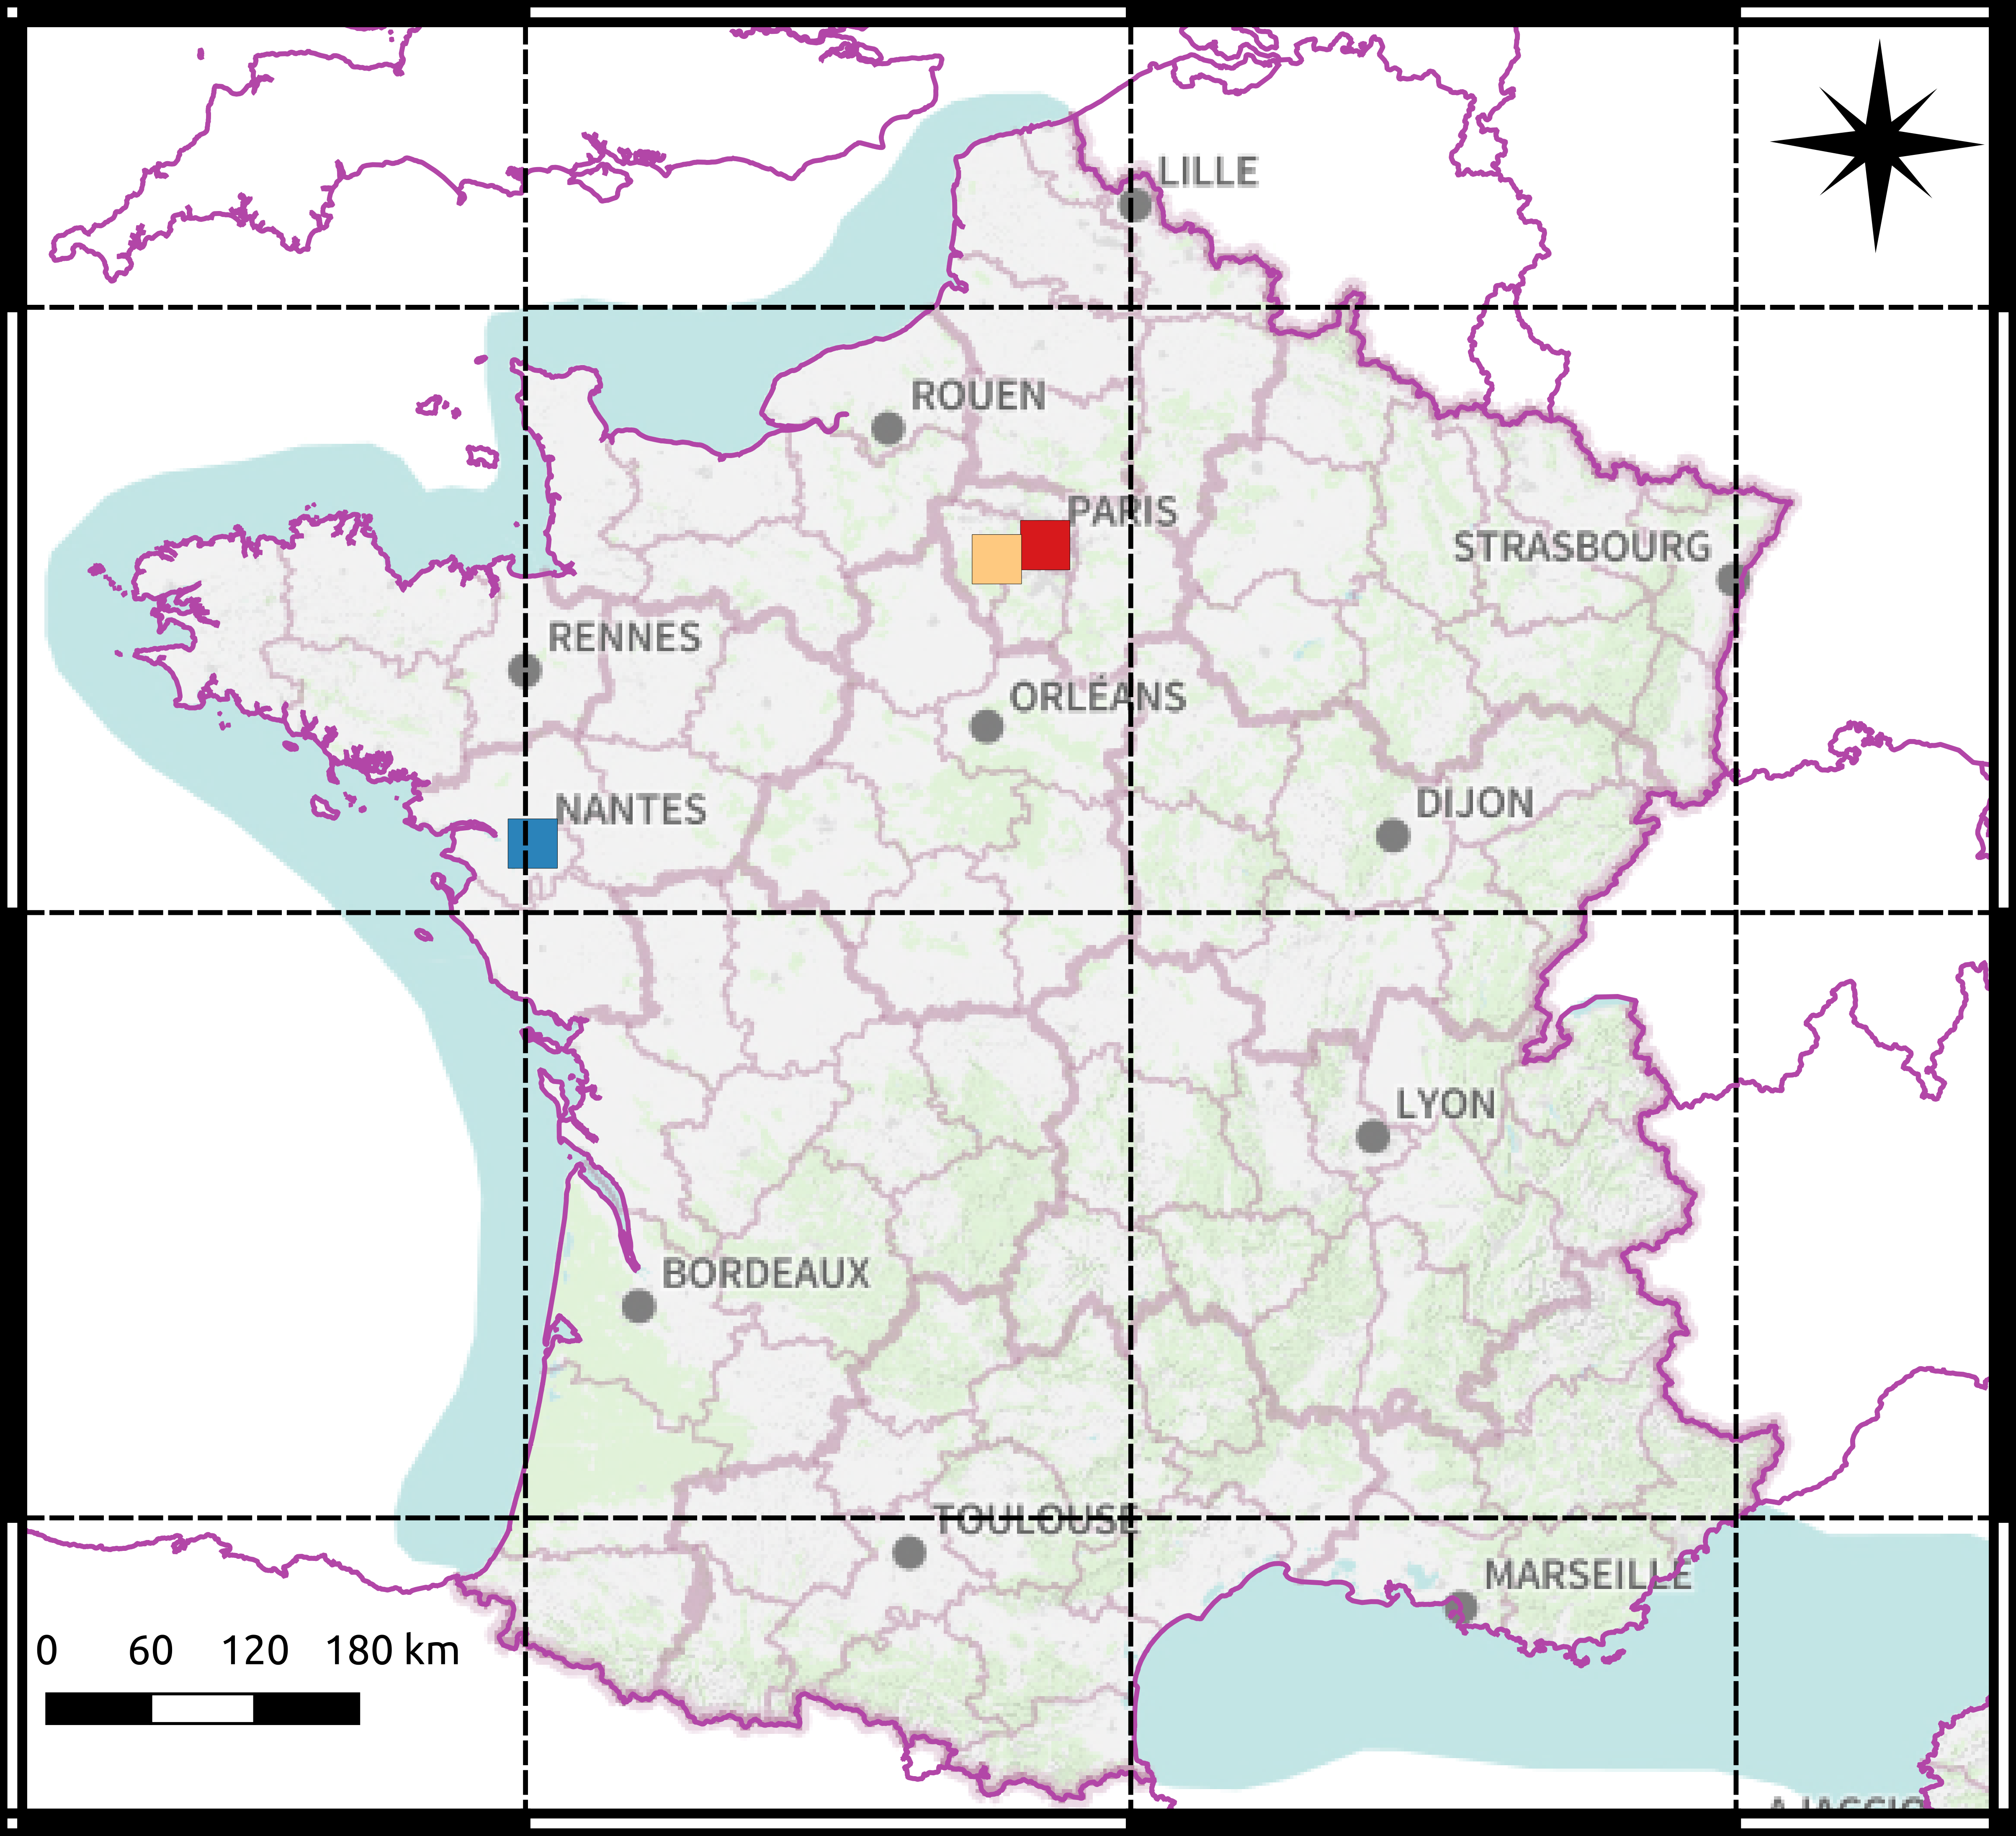
\includegraphics[height=.8\textheight]{images/datasets/france_map}
                }
                \only<2->{
                    \footnotesize
                    \begin{tabular}{c x{3cm} x{3cm}}
                        \toprule
                        & Elancourt & Na-P13 \\
                        \midrule
                        Algorithm & \multicolumn{2}{c}{Bati3D\textsuperscript{\textregistered}} \\
                        \midrule
                        \# samples & \num{2009} & \num{1226} \\
                        \midrule
                        Scene & residential \& industrial & dense downtown \& skyscrappers \\
                        \midrule
                        Image resolution & \SI{0.06}{\m} & \SI{0.1}{\m} \\
                        \bottomrule
                    \end{tabular}
                }
            \end{frame}

        \subsection{Results}
            \begin{frame}{Vanilla experiment}
                \includestandalone[mode=buildnew, height=.75\textheight]{figures/experiments/vanilla}
            \end{frame}

            \begin{frame}{Vanilla results}
                \includestandalone[mode=buildnew, height=.65\textheight]{figures/results/vanilla}

                \begin{itemize}[label=$\blacktriangleright$, font=\color{IGNGreen}]
                    \item \texttt{Building errors} on dense scenes: Still to be improved.
                    \item \texttt{Facet errors} always well detected.
                \end{itemize}
            \end{frame}

            \begin{frame}{Transferability experiment}
                \includestandalone[mode=buildnew, height=.65\textheight]{figures/experiments/transferability}
            \end{frame}

            \begin{frame}{Transferability results}
                \includestandalone[mode=buildnew, height=.65\textheight]{figures/results/transferability}
                
                \begin{itemize}[label=$\blacktriangleright$, font=\color{IGNGreen}]
                    \item<only@1> All errors > \SI{75}{\percent}.
                    \item<only@1> Except \texttt{\acrshort{acr::fib}} on \textbf{Elancourt}.
                    \item<only@2> Compared to \texttt{Vanilla}.
                    \item<only@2> Always better to train on \textbf{Elancourt}.
                \end{itemize}
            \end{frame}

    \section{Conclusion}
        \begin{frame}{Summary}
            \begin{itemize}[label=\(\blacktriangleright\), font=\color{IGNGreen}]
                \item<1-> \textbf{Hierarchical and modular} error taxonomy;
                \item<2-> \textbf{Scalable} evaluation method;
                \item<3-> Intrinsic features could be used for error prediction;
                \item<4-> Extrinsinc modalities \(\implies\) better transferability.
                \item<5-> An efficient building representation \(\implies\) even better transferability.
            \end{itemize}
        \end{frame}

    \bgroup
    \setbeamercolor{background canvas}{bg=white}

    \begin{frame}[plain]{}
        \newgeometry{top=0cm, left=0cm, right=0cm, bottom=0cm}
        \hspace{-.75cm}
        \begin{tikzpicture}
            \node (ign_logo) at (-1, 0) {
                
\includegraphics[width=1.606911447cm]{images/logos/logo-ign}
            };
            \path (ign_logo.south) node[anchor=north] (inria_logo) {
                
\includegraphics[width=1.606911447cm]{images/logos/logo-inria}
            };
            \path (ign_logo.north east) + (3, 0) node[anchor=north west] (trame) {\usebox \tramebox};
            \path (inria_logo.south west) + (0, -2.25) node[anchor=north west] (background) {
                {
                    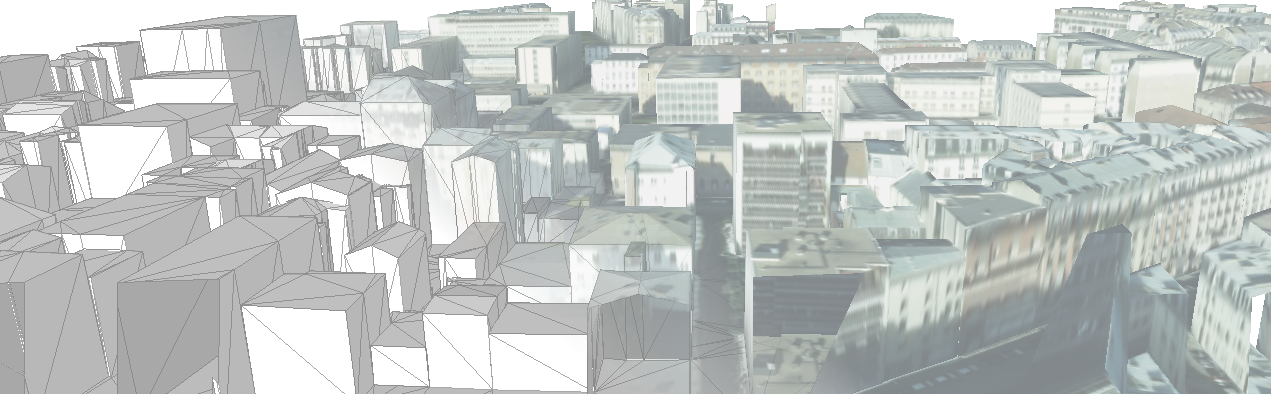
\includegraphics[width=11.5cm]{images/logos/background-50}
                }
            };
            \path (trame.west) + (2.5, -.75) node (title_box) {\usebox \titlebox};
            \path (title_box) + (0, .75) node (thanks) {
                \begin{beamercolorbox}[
                    wd=4cm,
                    sep=8pt
                ]{title page header}
                    \usebeamerfont{title}
                    \begin{center}
                        Thank you for your attention!
                    \end{center}
                \end{beamercolorbox}
            };
            \path (background.north) node[anchor=north] (author) {
                \begin{beamercolorbox}[
                    wd=4cm,
                    sep=8pt
                ]{author}
                    \usebeamerfont{author}
                    \begin{center}
                        \insertauthor\par
                    \end{center}
                \end{beamercolorbox}
            };
            \end{tikzpicture}
        \restoregeometry 
    \end{frame}
    \egroup

    \section*{Bonus}
        \subsection*{3D building models}
            \begin{frame}{\texorpdfstring{\acrshort*{acr::3d}}{3D} models}{More than pure geometry}
                \centering
                \includestandalone[mode=buildnew, height=.6\textheight]{figures/model_information}\\
                \begin{itemize}[label=\(\blacktriangleright\), font=\color{IGNGreen}]
                    \item \acrshort{acr::3d} model = \only<1>{\textbf{Geometry}}\only<2>{Geometry + \textbf{Topology}}\only<3->{Geometry + Topology + \textbf{Semantics}.}
                \end{itemize}
            \end{frame}

            \begin{frame}{Different levels of representation}
                \begin{figure}[H]
                    \centering
                    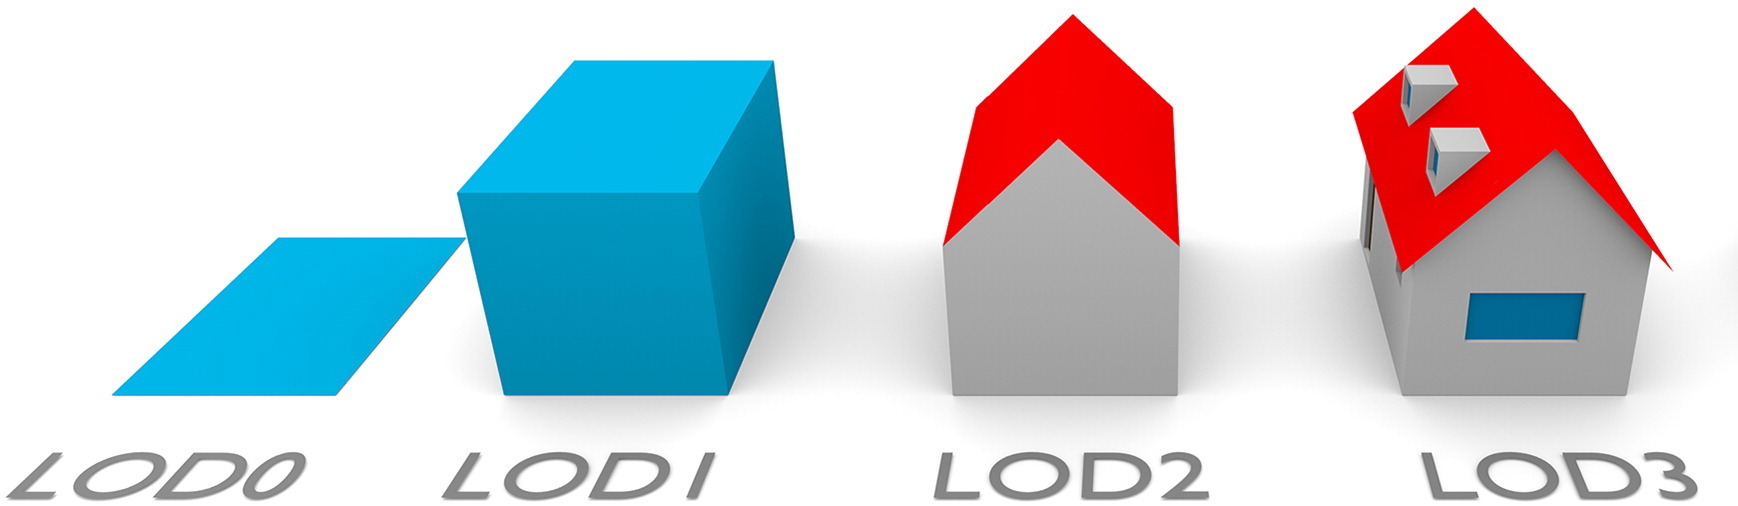
\includegraphics[width=\textwidth]{images/lods_3}
                    \caption{\acrshort{acr::lod} considered in the study~\parencite{biljecki2016improved}.}
                \end{figure}
                \vfill
                \uncover<2->{
                    Model \Acrfull{acr::lod} depends on:
                    \begin{itemize}[label=\(\blacktriangleright\), font=\color{IGNGreen}]
                        \item<3-> End user requirements;
                        \item<3-> Input data.
                    \end{itemize}
                }
            \end{frame}

        \subsection*{Error taxonomy}     
            \begin{frame}{Error classification}
                \includestandalone[mode=buildnew, width=\textwidth]{figures/taxonomy_tree_animated}
            \end{frame}

        \subsection*{Graph kernels}
            \begin{frame}{Graph kernels}
                \centering
                \includestandalone[mode=buildnew, width=\textwidth]{figures/features/geometric/kernels_menu_all}
            \end{frame}

        \subsection*{ScatNet}
            \begin{frame}{Our needs}
                \begin{itemize}[label=$\blacktriangleright$, font=\color{IGNGreen}]
                    \item<1-> Global feature vector per image.
                    \item<2-> Handles:
                    \begin{itemize}[label=$\blacktriangleright$, font=\color{IGNGreen}]
                        \item<2-> both depth and RGB images.
                        \item<3-> edges \& textures.
                        \item<4-> small dataset.
                    \end{itemize}
                \end{itemize}
                \vfill
                \uncover<5->{
                    Proposed solution: \Acrfull{acr::scatnet}~\parencite{mallat2012group}.
                }
            \end{frame}

            \begin{frame}{\texorpdfstring{\acrshort*{acr::scatnet}}{ScatNet} vs. \texorpdfstring{\acrshort*{acr::cnn}}{ConvNet}}
                \begin{itemize}[label=\(\blacktriangleright\), font=\color{IGNGreen}]
                    \item<1-> Filters are hardcoded not learned:
                    \begin{itemize}
                        \item[\color{IGNDarkGreen} +]<2-> No need for a large dataset;
                        \item[\color{IGNDarkGreen} +]<3-> Interpretable; 
                        \item[\color{IGNRed} ---]<4-> Features: not adaptable.
                    \end{itemize}
                    \item<5-> Limited to shallow layers:
                    \begin{itemize}
                        \item[\color{IGNRed} ---]<6-> Less powerful~\parencite{oyallon2015deep}.
                    \end{itemize}
                \end{itemize}
            \end{frame}

            \begin{frame}{\texorpdfstring{\acrshort*{acr::scatnet}}{ScatNet}}
                \begin{itemize}[label=\(\blacktriangleright\), font=\color{IGNGreen}]
                    \item<1-> Reverse engineered \acrfull{acr::cnn}~\parencite{mallat2012group};
                    \item<2-> Ingredients: 
                    \begin{itemize}[label=\(\blacktriangleright\), font=\color{IGNGreen}]
                        \item<3-> Band pass filters \(\longrightarrow\) high frequency information~\parencite{sifre2013rotation};
                        \item<4-> Modulus \(\longrightarrow\) non-linearity~\parencite{anden2014deep};
                        \item<5-> Average pooling operator \(\longrightarrow\) local invariance~\parencite{mallat2012group}.
                    \end{itemize}
                \end{itemize}
                \begin{overlayarea}{\textwidth}{.3\textheight}
                    \centering
                    \only<3>{
                        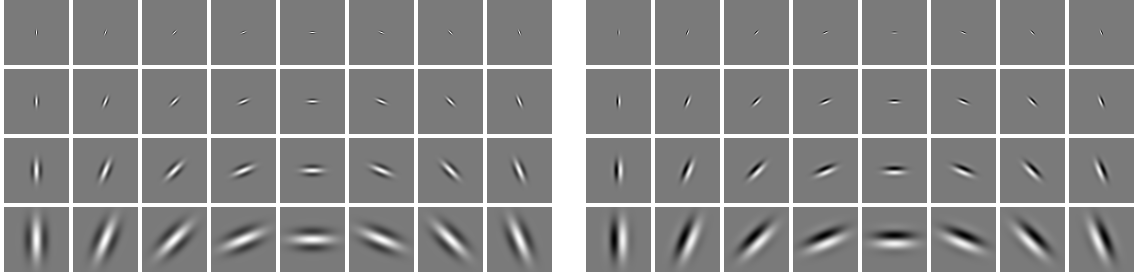
\includegraphics[width=\textwidth]{images/scatnet/morlet_wavelets}
                    }
                \end{overlayarea}
            \end{frame}

            \begin{frame}{\texorpdfstring{\acrshort*{acr::scatnet}}{ScatNet} structure}
                \centering
                \includestandalone[mode=buildnew, height=.8\textheight]{figures/features/scattering_networks}
            \end{frame}

            \begin{frame}{\texorpdfstring{\acrshort*{acr::scatnet}}{ScatNet} filters}
                \centering
                \only<1>{
                    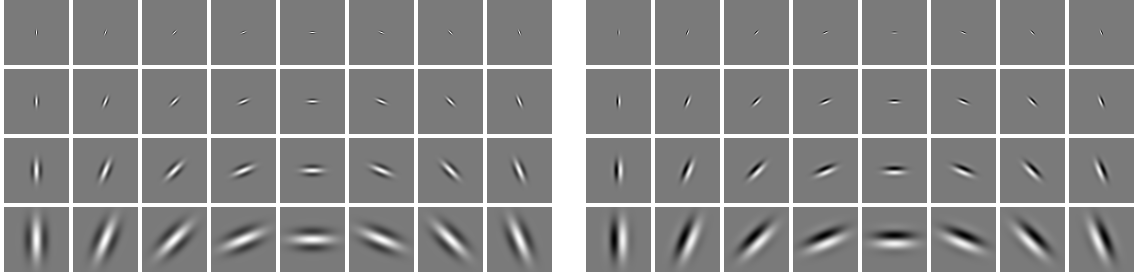
\includegraphics[width=\textwidth]{images/scatnet/morlet_wavelets}
                }
                \only<2>{
                    
\includegraphics[width=.35\textwidth]{images/scatnet/first_layer_cnn}\\
                    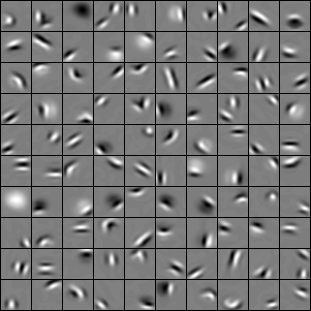
\includegraphics[width=.5\textwidth]{images/scatnet/second_layer_cnn}
                }
            \end{frame}

        \subsection*{Dataset}
            \begin{frame}{Error statistics}
                \framesubtitle<1>{\texttt{finesse}=2}
                \framesubtitle<2>{\texttt{Building errors}}
                \framesubtitle<3>{\texttt{Facet errors}}
                \framesubtitle<4->{Summary}

                \centering
                \only<1>{
                    \includestandalone[mode=buildnew, height=.75\textheight]{figures/datasets/families_stats_animated}
                }
                \only<2>{
                    \includestandalone[mode=buildnew, height=.75\textheight]{figures/datasets/lod1_stats_animated}
                }
                \only<3>{
                    \includestandalone[mode=buildnew, width=\textwidth]{figures/datasets/lod2_stats_animated}
                }
                \only<4->{
                    \begin{itemize}[label=$\blacktriangleright$, font=\color{IGNGreen}]
                        \item Highly unbalanced data;
                        \item Dense scenes (\textbf{Nantes} \& \textbf{Paris-13}):
                        \begin{itemize}[label=\(\rightarrow\)]
                            \item High \texttt{Facet errors} count;
                            \item Low \texttt{Building errors} count;
                        \end{itemize}
                        \item Sparce scene: inverse.
                    \end{itemize}
                }
            \end{frame}

        \subsection*{Setup}
            \begin{frame}{Parameters}
                \begin{itemize}[label=$\blacktriangleright$, font=\color{IGNGreen}]
                    \small
                    \item<1-> \Acrfull{acr::rf}:
                    \begin{description}
                        \item<2->[Max depth] \num{4};
                        \item<2->[Number of trees] \num{1000};
                    \end{description}
                    \item<3-> \Acrfull{acr::svm}:
                    \begin{description}
                        \item<4->[Slack pen.] \num{.1};
                        \item<4->[\gls{acr::rbf}] \(\gamma\) = \num{.001};
                        \item<4->[\gls{acr::mkl}] EasyMKL.
                    \end{description}
                    \item<5-> Feature configurations:
                    \begin{itemize}
                        \item<6-> \textbf{(K-)Geom.};
                        \item<6-> \textbf{(K-)Geom.} \(\oplus\) \textbf{S-Hei.};
                        \item<6-> \textbf{(K-)Geom.} \(\oplus\) \textbf{S(d)-Im.};
                        \item<6-> \textbf{(K-)Geom.} \(\oplus\) \textbf{S(c)-Im.};
                        \item<6-> \textbf{(K-)S(d)-All} = \textbf{(K-)Geom.} \(\oplus\) \textbf{S-Hei.} \(\oplus\) \textbf{S(d)-Im.}.
                        \item<6-> \textbf{(K-)S(c)-All} = \textbf{(K-)Geom.} \(\oplus\) \textbf{S-Hei.} \(\oplus\) \textbf{S(c)-Im.}.
                    \end{itemize}
                \end{itemize}
            \end{frame}

            \begin{frame}{Possible settings}
                \centering
                \footnotesize
                \begin{tabular}{c c c c c}
                    \toprule
                    Features & Classifier & Experiment & \texttt{finesse} & Configurations\\
                    \hline
                    \multirow{2}{*}{Baseline} & \acrshort{acr::rf} & \multirow{6}{*}{Vanilla} & \multirow{10}{*}{3} & \num{4 x 1} \\
                     & \acrshort{acr::svm} &  &  & \num{4 x 2} \\
                    \cline{1-2}
                    \multirow{2}{*}{\gls{acr::scatnet}} & \acrshort{acr::rf} &  &  & \cellcolor{IGNGreen}<2>{\num{6 x 2}} \\
                     & \acrshort{acr::svm} &  &  & \cellcolor{IGNGreen}<2>{\num{6 x 2}} \\
                    \cline{1-2}
                    Graph Kernels & \acrshort{acr::svm} &  &  & \cellcolor{IGNGreen}<2>{\num{1 x 2}} \\
                    \cline{1-2}
                    GK \(\oplus\) \gls{acr::scatnet} & \acrshort{acr::svm} &  &  & \cellcolor{IGNGreen}<2>{\num{6 x 2}} \\
                    \cline{1-3}
                    \multirow{2}{*}{\gls{acr::scatnet}} & \acrshort{acr::rf} & \multirow{4}{*}{Transferability} & & \cellcolor{IGNGreen}<2>{\num{6 x 2}} \\
                     & \acrshort{acr::svm} &  &  & \cellcolor{IGNGreen}<2>{\num{6 x 2}} \\
                    \cline{1-2}
                    Graph Kernels & \acrshort{acr::svm} &  &  & \cellcolor{IGNGreen}<2>{\num{1 x 2}} \\
                    \cline{1-2}
                    GK \(\oplus\) \gls{acr::scatnet} & \acrshort{acr::svm} &  &  & \num{6 x 2} \\
                    \hline
                    \multicolumn{4}{l}{Total} & \num{88}\\
                    \bottomrule
                \end{tabular}
            \end{frame}

    \end{document}
